\documentclass[AnalisiDeiRequisiti.tex]{subfiles}

\begin{document}

\chapter{Casi d'uso}
\section{Attori dei casi d'uso}
\subsection{Attori primari}
\begin{enumerate}
	\begin{figure}[h]
		\centering
		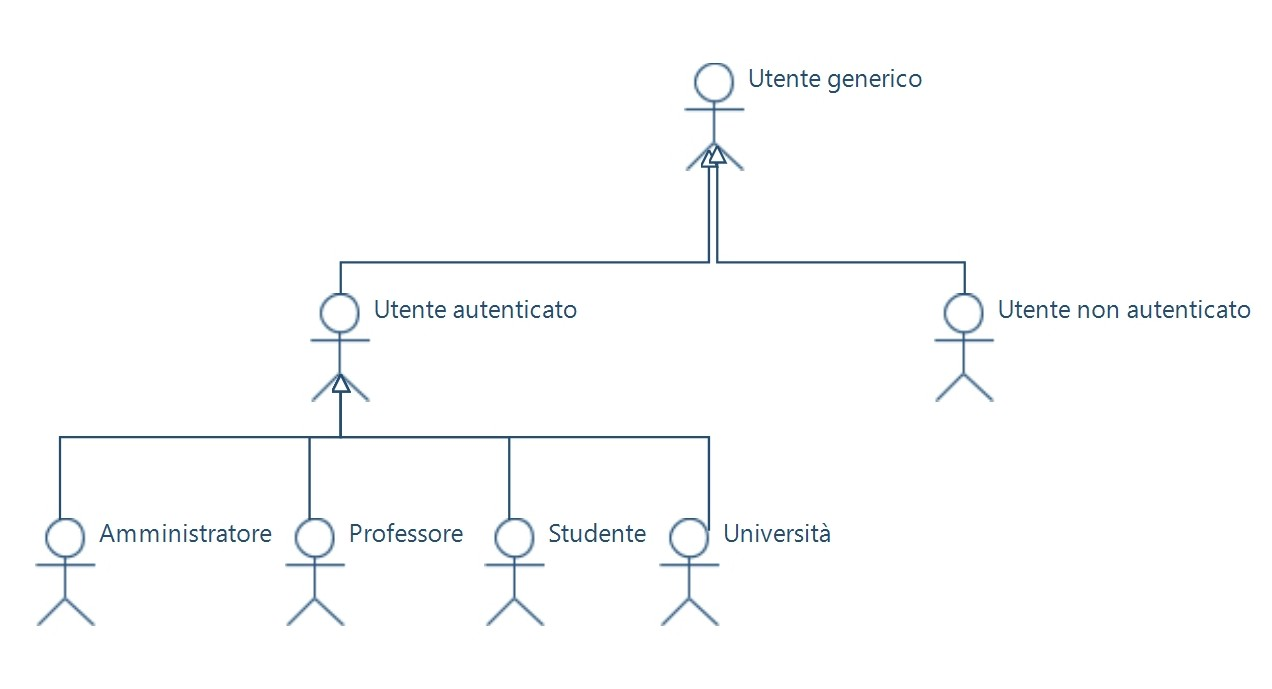
\includegraphics[width=0.8\linewidth]{attoriPrincipali.jpg}
		\caption{Gerarchia attori primari}
		\label{fig:Gerarchia attori primari}
	\end{figure}
	
	\item \textbf{Utente generico}\\
	Si riferisce ad un utente generico che accede al sito\\
	
	\item \textbf{Utente non autenticato}\\
	Ci si riferisce ad un utente generico con non ha ancora effettuato il login.\\
	
	\item \textbf{Utente autenticato}\\
	 Ci si riferisce ad un utente generico con chiave valida ed autenticato nel sistema tramite la procedura di login.\\
	
	\item \textbf{Amministratore}\\
	Ci si riferisce ad un utente autenticato nel sistema nel ruolo di amministratore\\
	
	\item \textbf{Professore}\\
	Ci si riferisce ad un utente autenticato nel sistema nel ruolo di professore.\\
	
	\item \textbf{Studente}\\
	Ci si riferisce ad un utente autenticato nel sistema nel ruolo di studente\\	
\end{enumerate}

\subsection{Attori secondari}
\begin{enumerate}
	\item \textbf{MetaMask}\\
	Plugin del browser MetaMask per interfacciarsi ad una rete Ethereum.\\
	
	\item \textbf{Ufficio Universitario}\\
	Entità fisica che consente l'immatricolazione e la registrazione dei professori.\\
\end{enumerate}

\section{Elenco dei casi d'uso}

\begin{figure}[H]
	\centering
	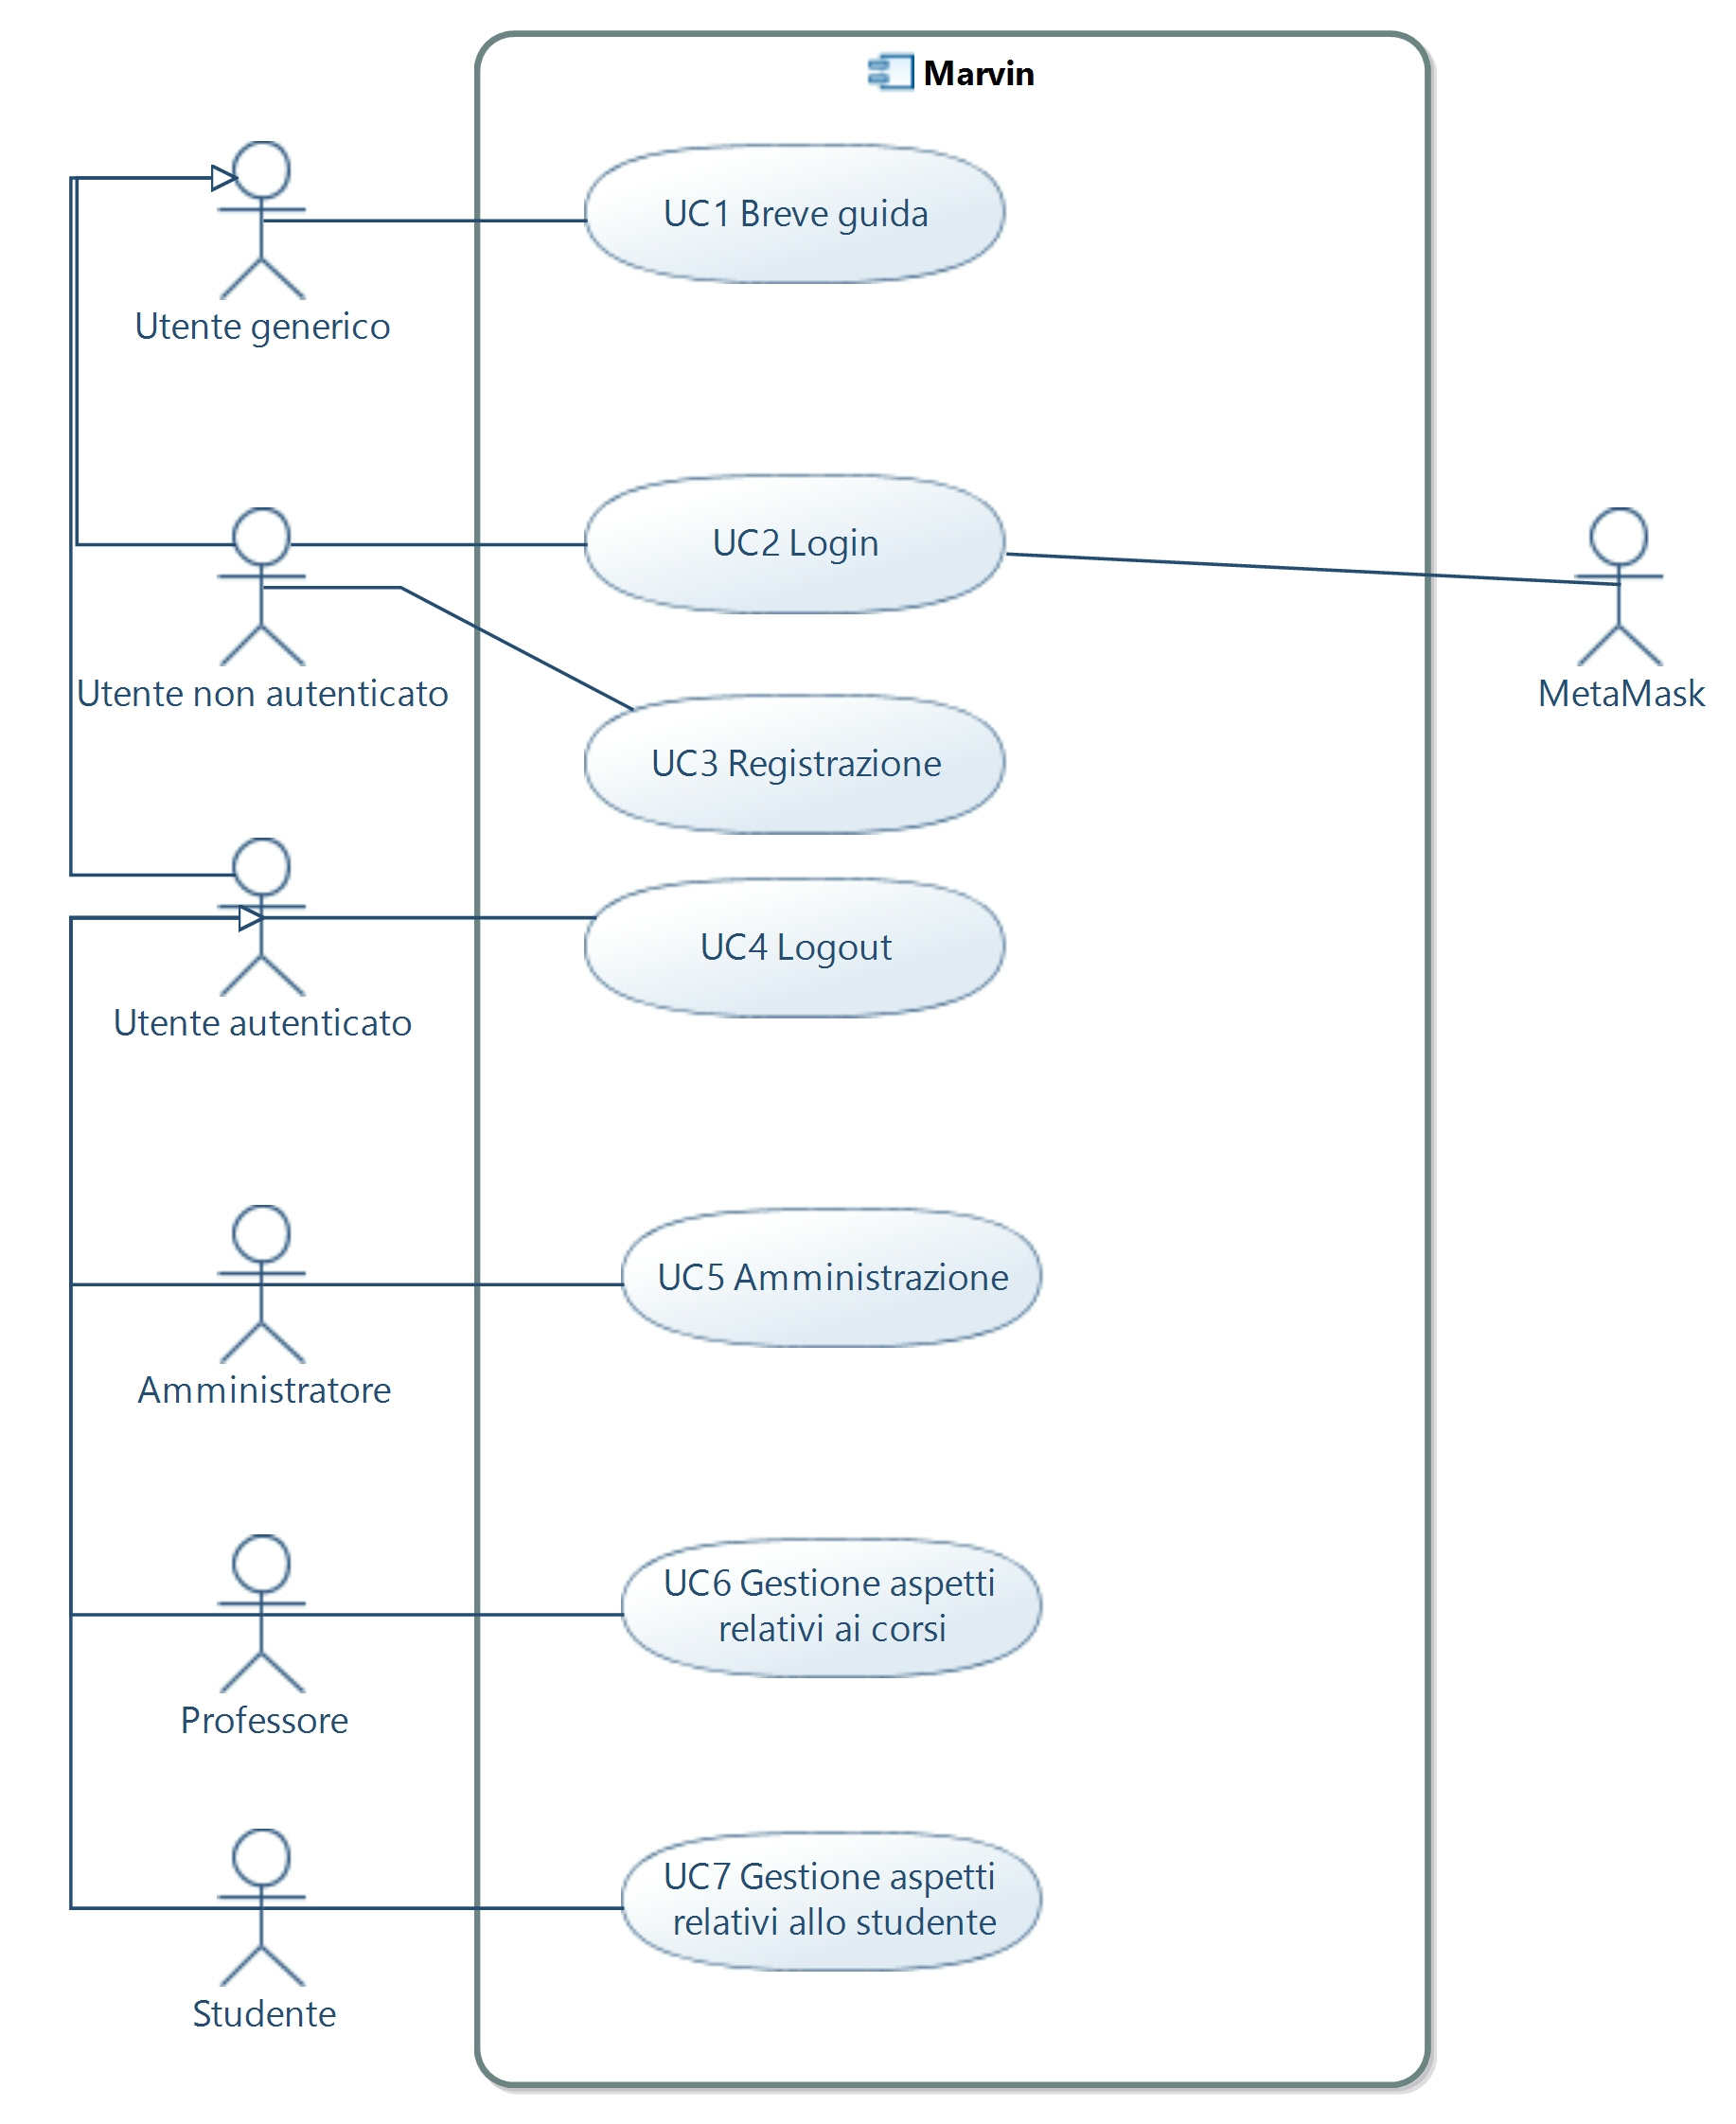
\includegraphics[width=0.8\linewidth]{UC.jpg}
	\caption{Casi d'uso basilari}
	\label{fig:Casi d'uso basilari}
\end{figure}

%   -------------------------------------------------------------------------------------
%   ----------                 MODELLO PER GLI USER CASE              -------------------
%   -------------------------------------------------------------------------------------
\begin{comment}
\subsection{UCX - Nome}
\begin{itemize}
	\item \textbf{Attori primari:} ;\\
	\item \textbf{Attori secondari:} ;\\
	\item \textbf{Scopo e descrizione:} ;\\
	\item \textbf{Scenario principale:} ;\\
	\item \textbf{Scenario alternativo:} ;\\
	\item \textbf{Flusso principale degli eventi:};\\
	\begin{enumerate}
		\item L'utente... ;
		\item L'utente... ;
	\end{enumerate}
	\item \textbf{Estensioni:}\\
		\begin{enumerate}
		\item Se l'utente... ;[UCX.X.X]
	\end{enumerate}
	\item \textbf{Precondizione:} ;\\
	\item \textbf{Postcondizione:} .\\
\end{itemize}
\end{comment}
%
\subsection{UC1 - Breve guida}
\begin{itemize}
	\item \textbf{Attori primari:} Utente generico;\\
	\item \textbf{Scopo e descrizione:} L'utente visualizza una breve guida di introduzione su come installare il plugin MetaMask e su come gestire le chiavi in modo da istruirlo sulle modalità di accesso al sistema;\\
	\item \textbf{Scenario principale:} L'utente accede alla guida;\\
	\item \textbf{Precondizione:} Il sistema è raggiungibile e funzionante e l'utente desidera aprire la guida;\\
	\item \textbf{Postcondizione:} L'utente ha avuto delle nozioni riguardanti l'accesso al sistema.\\
\end{itemize}
\subsection{UC2 - Login}
\begin{itemize}
	\item \textbf{Attori primari} Utente non autenticato;\\
	\item \textbf{Scopo e descrizione:} L'utente richiede il login al sistema attraverso il plugin MetaMask;\\
	\item \textbf{Scenario principale:} L'utente non ancora riconosciuto dal sistema effettua il login;\\
	\item \textbf{Precondizione:} L'utente non è stato riconosciuto dal sistema;\\
	\item \textbf{Postcondizione:} L'utente viene riconosciuto da parte del sistema.\\
\end{itemize}

\begin{figure}[H]
	\centering
	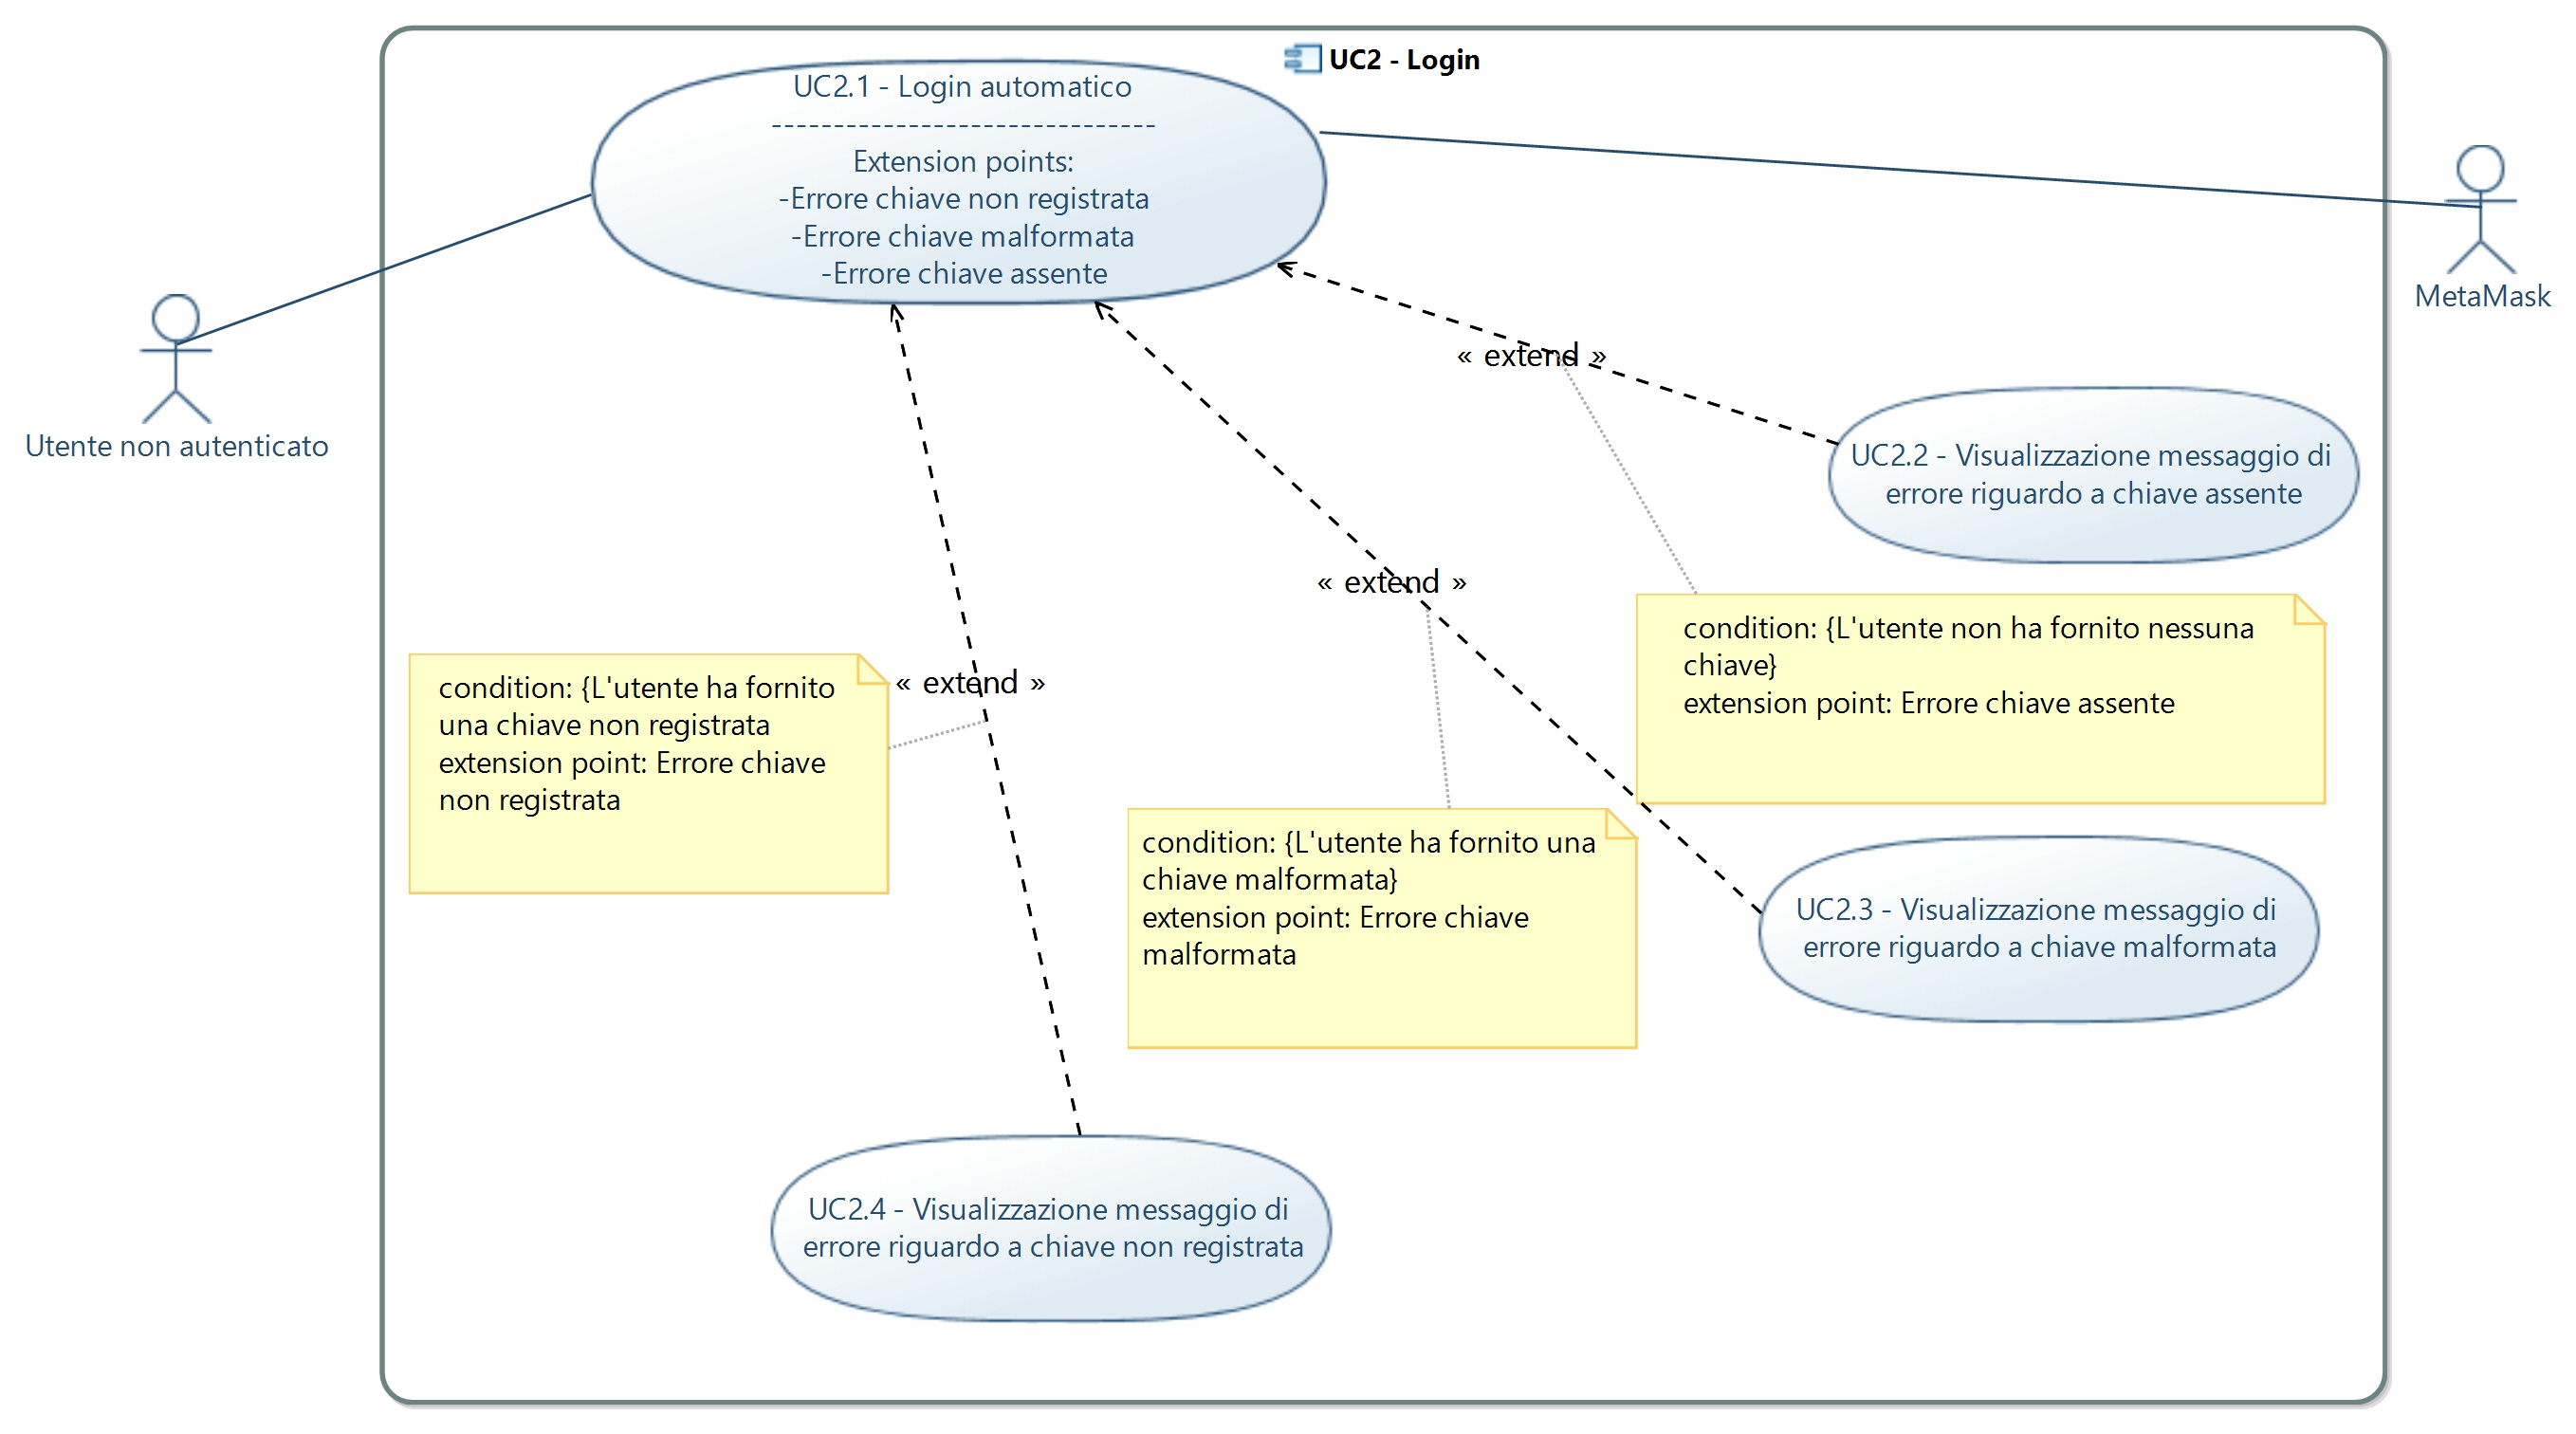
\includegraphics[width=1.0\linewidth]{UC2.jpg}
	\caption{UC2 - Login}
	\label{fig:UC2 - Login}
\end{figure}

\subsection{UC2.1 - Login automatico}
\begin{itemize}
\item \textbf{Attori primari} Utente non autenticato;\\
\item \textbf{Attori secondari:} MetaMask;\\
\item \textbf{Scopo e descrizione:} L'utente attende il login da parte del sistema senza effettuare nessuna operazione aggiuntiva;\\
\item \textbf{Scenario principale:} L'utente non ancora riconosciuto dal sistema richiede il login;\\
\item \textbf{Estensioni:}\\
\begin{enumerate}
	\item Se l'utente non ha a disposizione una chiave viene avvisato con un errore a riguardo [UC2.2];
	\item Se l'utente ha a disposizione una chiave malformata viene avvisato con un errore a riguardo [UC2.3];
	\item Se l'utente ha a disposizione una chiave non registrata viene avvisato con un errore a riguardo [UC2.4];
\end{enumerate}
\item \textbf{Precondizione:} L'utente ha richiesto al sistema di venire riconosciuto;\\
\item \textbf{Postcondizione:} L'utente viene riconosciuto da parte del sistema.\\
\end{itemize}
\subsection{UC2.2 - Visualizzazione messaggio di errore riguardo a chiave assente}
\begin{itemize}
	\item \textbf{Attori primari:} Utente non autenticato;\\
	\item \textbf{Scopo e descrizione:} L'utente viene avvisato del fatto che non ha fornito nessuna chiave al sistema;\\
	\item \textbf{Scenario principale:} L'utente visualizza l'errore relativo all'assenza di una chiave per accedere al sistema;\\
	\item \textbf{Precondizione:} L'utente richiede il login senza fornire una chiave;\\
	\item \textbf{Postcondizione:} L'utente è consapevole di dover fornire una chiave. \\
\end{itemize}
\subsection{UC2.3 - Visualizzazione messaggio di errore riguardo a chiave malformata}
\begin{itemize}
	\item \textbf{Attori primari:} Utente non autenticato;\\
	\item \textbf{Scopo e descrizione:} L'utente viene avvisato del fatto che ha fornito una chiave malformata, quindi con lunghezza invalida o contenente caratteri non permessi;\\
	\item \textbf{Scenario principale:} L'utente visualizza il messaggio d'errore relativo alla chiave malformata;\\
	\item \textbf{Precondizione:} L'utente richiede il login utilizzando una chiave malformata;\\
	\item \textbf{Postcondizione:} L'utente è consapevole di cambiare la chiave o sistemare quella fornita.\\
\end{itemize}
\subsection{UC2.4 - Visualizzazione messaggio di errore riguardo a chiave non registrata}
\begin{itemize}
	\item \textbf{Attori primari:} Utente non autenticato;\\
	\item \textbf{Scopo e descrizione:} L'utente viene avvisato del fatto che ha fornito una chiave non registrata nel sistema;\\
	\item \textbf{Scenario principale:} L'utente viene informato che la sua chiave non risulta registrata, suggerendone la registrazione;\\
	\item \textbf{Precondizione:} L'utente richiede il login utilizzando una chiave non registrata;\\
	\item \textbf{Postcondizione:} L'utente è consapevole di dover effettuare la registrazione per accedere al sistema.\\
\end{itemize}
%TODO Grafico UC3
\subsection{UC3 - Registrazione}
\begin{itemize}
	\item \textbf{Attori primari:} Utente non autenticato;\\
	\item \textbf{Scopo e descrizione:} L'utente compila i campi richiesti per registrarsi nel sistema;\\
	\item \textbf{Scenario principale:}
	\begin{enumerate}
		\item L'utente inserisce il suo nome[UC3.1];
		\item L'utente inserisce il suo cognome [UC3.2];
		\item L'utente seleziona la sua categoria [UC3.3]
		\item L'utente seleziona il corso desiderato [UC3.4]
	\end{enumerate}
	\item \textbf{Estensioni:}
	\begin{enumerate}
		\item Se l'utente non compila uno dei campi viene mostrato un messaggio che suggerisce la compilazione del campo mancante [UC3.5]
	\end{enumerate}
	\item \textbf{Precondizione:} L'utente è entrato nel sistema e ha scelto di registrarsi;\\
	\item \textbf{Postcondizione:} La registrazione è andata a buon fine e la chiave dell'utente è stata salvata nel sistema.\\
\end{itemize}
\subsection{UC3.1 - Inserimento nome}
\begin{itemize}
	\item \textbf{Attori Primari:} Utente non autenticato;
	\item \textbf{Scopo e Descrizione} Il sistema offre l'interfaccia per inserire il nome dell'utente;
	\item \textbf{Scenario principale:} L'utente fornisce tramite un dispositivo di input il suo nome;
	\item \textbf{Precondizione:} Il sistema offre un campo per la compilazione del nome e rimane in attesa dell'input;
	\item \textbf{Postcondizione:} L'utente ha inserito nome nel campo fornito dal sistema;
\end{itemize}	
\subsection{UC3.2 - Inserimento cognome}
\begin{itemize}
	\item \textbf{Attori Primari:} Utente non autenticato;
	\item \textbf{Scopo e Descrizione} Il sistema offre l'interfaccia per inserire il cognome dell'utente;
	\item \textbf{Scenario principale:} L'utente fornisce tramite un dispositivo di input il suo cognome;
	\item \textbf{Precondizione:} Il sistema offre un campo per la compilazione del cognome e rimane in attesa dell'input.;
	\item \textbf{Postcondizione:} L'utente ha inserito il suo cognome nel campo fornito dal sistema;
\end{itemize}
\subsection{UC3.3 - Selezione categoria}
\begin{itemize}
	\item \textbf{Attori Primari:} Utente non autenticato;
	\item \textbf{Scopo e Descrizione} Il sistema offre l'interfaccia per selezionare la categoria di registrazione (studente o professore);
	\item \textbf{Scenario principale:} L'utente seleziona tramite un dispositivo di input la sua categoria;
	\item \textbf{Precondizione:} Il sistema offre un campo per la selezione della categoria e rimane in attesa dell'input;
	\item \textbf{Postcondizione:} L'utente ha selezionato la sua categoria nel campo fornito dal sistema;
\end{itemize}
\subsection{UC3.4 - Selezione corso}
\begin{itemize}
	\item \textbf{Attori Primari:} Utente non autenticato;
	\item \textbf{Scopo e Descrizione} Il sistema offre l'interfaccia per selezionare il corso di laurea desiderato;
	\item \textbf{Scenario principale:} L'utente seleziona tramite un dispositivo di input il corso di laurea scelto;
	\item \textbf{Precondizione:} L'utente ha selezionato la registrazione come studente, il sistema offre un campo per la selezione del corso di laurea e rimane in attesa dell'input;
	\item \textbf{Postcondizione:} L'utente ha selezionato il suo corso di laurea nel campo fornito dal sistema;
\end{itemize}
\subsection{UC3.5 - Visualizzazione errore campo non compilato}
\begin{itemize}
	\item \textbf{Attori Primari:} Utente non autenticato;
	\item \textbf{Scopo e Descrizione} Il sistema avvisa l'utente che non ha compilato tutti i campi necessari per la registrazione al sistema;
	\item \textbf{Scenario principale:} Il sistema mostra un messaggio d'errore all'utente che indica di compilare i campi mancanti;
	\item \textbf{Precondizione:} L'utente tenta di registrarsi senza compilare tutti i campi;
	\item \textbf{Postcondizione:} L'utente è consapevole di non aver compilato tutti i campi;
\end{itemize}
\subsection{UC4 - Logout}
\begin{itemize}
	\item \textbf{Attori primari:} Utente Autenticato;
	\item \textbf{Attori secondari:} Metamask;
	\item \textbf{Scopo e descrizione:} L'utente effettua il logout dal sistema tramite il plugin Metamask;
	\item \textbf{Scenario principale:} L'utente autenticato richiede il logout dal sistema;
	\item \textbf{Precondizione:} L'utente è autenticato e vuole effettuare il logout;
	\item \textbf{Postcondizione:} L'utente non è più riconosciuto dal sistema.
\end{itemize}
\subsection{UC5 - Amministrazione}
\begin{itemize}
	\item \textbf{Attori primari:} Amministratore;
	\item \textbf{Scopo e descrizione:} L'amministratore è nella sua area personale e ottiene una lista di azioni da compiere;
	\item \textbf{Scenario principale:} L'utente visualizza le azioni che può compiere e ne sceglie una; 
	\item \textbf{Precondizione:} L'utente è riconosciuto dal sistema come amministratore e vuole eseguire delle operazioni; 
	\item \textbf{Postcondizione:} L'utente è a conoscenza delle azioni che può eseguire e ne ha scelta una.
\end{itemize}
\subsection{UC5.1 - Gestione Studenti}
\begin{itemize}
	\item \textbf{Attori primari:} Amministratore;
	\item \textbf{Scopo e descrizione:} L'utente è in grado di eseguire operazioni sugli studenti all'interno dell'ateneo;
	\item \textbf{Scenario principale:} L'utente visualizza una lista di operazioni eseguibili sugli studenti e sceglie quale fare;
	\item \textbf{Precondizione:} L'utente ha scelto di gestire gli studenti; 
	\item \textbf{Postcondizione:}L'utente è a conoscenza delle operazioni che può eseguire sugli studenti e decide di effettuarne una.
\end{itemize}
\subsection{UC5.1.1 - Visualizzazione lista di studenti}
\begin{itemize}
	\item \textbf{Attori primari:} Amministratore;
	\item \textbf{Scopo e descrizione:} L'utente visualizza una lista di tutti gli studenti registrati nel sistema;
	\item \textbf{Scenario principale:} L'utente richiede al sistema una lista di studenti per poterli gestire;
	\item \textbf{Precondizione:} L'utente è nell'area di gestione studenti e richiede una lista di tutti gli studenti; 
	\item \textbf{Postcondizione:} L'utente ottiene la lista.
\end{itemize}
\subsection{UC5.1.2 - Visualizzazione lista di studenti non approvati}
\begin{itemize}
	\item \textbf{Attori primari:} Amministratore;
	\item \textbf{Scopo e descrizione:} L'utente visualizza una lista di tutti gli studenti ancora non approvati;
	\item \textbf{Scenario principale:} L'utente richiede al sistema una lista di studenti non approvati per poterli gestire;
	\item \textbf{Precondizione:}L'utente è nell'area di gestione studenti e richiede una lista di studenti non approvati; 
	\item \textbf{Postcondizione:} L'utente ottiene la lista.
\end{itemize}
\subsection{UC5.1.3 - Approvazione Studente}
\begin{itemize}
	\item \textbf{Attori primari:} Amministratore;
	\item \textbf{Scopo e descrizione:} L'utente approva la registrazione dello studente;
	\item \textbf{Scenario principale:}
	\begin{enumerate}
		\item L'utente seleziona uno studente non ancora approvato;
		\item L'utente lo approva
	\end{enumerate}
	\item \textbf{Precondizione:} L'utente ha richiesto una lista di studenti non approvati; 
	\item \textbf{Postcondizione:} Lo studente selezionato viene approvato e il suo stato viene aggiornato nel sistema.
\end{itemize}
\subsection{UC5.1.4 - Cambio corso di laurea}
\begin{itemize}
	\item \textbf{Attori primari:} Amministratore;
	\item \textbf{Scopo e descrizione:} L'utente cambia il corso di laurea a cui è associato uno studente;
	\item \textbf{Scenario principale:}
	\begin{enumerate}
		\item L'utente seleziona uno studente con o senza corso di laurea;
		\item L'utente seleziona un corso di laurea e lo associa allo studente
	\end{enumerate}
	\item \textbf{Precondizione:} L'utente ha richiesto una lista completa di studenti e vuole cambiare il corso di laurea ad uno di questi; 
	\item \textbf{Postcondizione:} Allo studente selezionato viene associato il nuovo corso di laurea nel sistema.
\end{itemize}
\subsection{UC5.3 - Gestione Anni Accademici}
\begin{itemize}
	\item \textbf{Attori primari:} Amministratore;
	\item \textbf{Scopo e descrizione:} L'utente è in grado di eseguire operazioni sugli anni accademici dell'ateneo;
	\item \textbf{Scenario principale:} L'utente visualizza una lista di operazioni eseguibili sugli anni accademici e ne sceglie una;
	\item \textbf{Precondizione:} L'utente ha scelto di gestire gli anni accademeici; 
	\item \textbf{Postcondizione:} L'utente è a conoscenza delle possibili operazioni da eseguire sugli anni accademici e ne ha scelta una.
\end{itemize}
\subsection{UC5.3.1 - Aggiunta Anno Accademico}
\begin{itemize}
	\item \textbf{Attori primari:} Amministratore;
	\item \textbf{Scopo e descrizione:} L'utente aggiunge un anno accademico nel sistema;
	\item \textbf{Scenario principale:} L'utente inserisce il numero dell'anno da aggiungere in un campo fornito dal sistema;
	\item \textbf{Estensioni:}
	\begin{enumerate}
		\item Se l'utente inserisce un'anno non numerico viene mostrato un messaggio d'errore relativo alla malformazione dell'anno;[UC5.1.4]
		\item Se l'utente inserisce un'anno già presente nel sistema viene mostrato un messaggio d'errore relativo alla non univocità dell'anno.[UC5.1.5]
		\item Se l'utente lascia il campo vuoto l'utente viene avvisato con un relativo messaggio d'errore.[UC5.1.6]
	\end{enumerate}
	\item \textbf{Precondizione:} L'utente ha scelto di aggiungere un anno accademico; 
	\item \textbf{Postcondizione:} L'anno accademico creato viene inserito nel sistema.
\end{itemize}
\subsection{UC5.3.2 - Visualizzazione lista di tutti gli anni accademici}
\begin{itemize}
	\item \textbf{Attori primari:} Amministratore;
	\item \textbf{Scopo e descrizione:} L'utente visualizza una lista di tutti gli anni accademici presenti nel sistema;
	\item \textbf{Scenario principale:} L'utente richiede la lista di tutti gli anni del sistema;
	\item \textbf{Precondizione:} L'utente p nell'area di gestione Anni Accademici e vuole ottenere la lista di tutti gli anni presenti nel sistema; 
	\item \textbf{Postcondizione:} L'utente ottiene la lista.
\end{itemize}
\subsection{UC5.3.3 - Aggiunta di un corso di laurea ad un anno accademico}
\begin{itemize}
	\item \textbf{Attori primari:} Amministratore;
	\item \textbf{Scopo e descrizione:} L'utente aggiunge un corso di laurea già presente nel sistema all'interno dell'anno accademico;
	\item \textbf{Scenario principale:}
	\begin{enumerate}
		\item L'utente seleziona l'anno accademico;
		\item L'utente ottiene una lista di corsi di laurea; [UC 5.4.1]
		\item L'utente seleziona il corso di laurea e lo inserisce all'interno dell'anno accademico.
	\end{enumerate}
	\item \textbf{Precondizione:} L'utente vuole aggiungere un corso di laurea all'anno accademico è ha ottenuto una lista degli anni accademici presenti nel sistema; 
	\item \textbf{Postcondizione:} Il corso di laurea è stato correlato con l'anno accademico e il loro stato è stato aggiornato nel sistema.
\end{itemize}
\subsection{UC5.3.4 - Visualizzazione messaggio anno malformato}
\begin{itemize}
	\item \textbf{Attori primari:} Amministratore;
	\item \textbf{Scopo e descrizione:} L'utente visualizza un messaggio che lo informa che l'anno inserito non è numerico;
	\item \textbf{Scenario principale:} Il sistema mostra all'utente un messaggio d'errore relativo alla malformazione dell'anno inserito;
	\item \textbf{Precondizione:} L'utente prova a creare un nuovo anno accademico inserendo un'anno non numerico; 
	\item \textbf{Postcondizione:} L'utente è consapevole di aver provato ad inserire un anno non numerico.
\end{itemize}
\subsection{UC5.3.5 - Visualizzazione messaggio di anno accademico già presente}
\begin{itemize}
	\item \textbf{Attori primari:} Amministratore;
	\item \textbf{Scopo e descrizione:} L'utente visualizza un messaggio che indica che un anno accademico come quello inserito è già presente nel sistema;
	\item \textbf{Scenario principale:} Il sistema mostra all'utente un messaggio d'errore relativo alla non univocità dell'anno accademico inserito;
	\item \textbf{Precondizione:} L'utente tenta di inserire un anno accademico già presente nel sistema; 
	\item \textbf{Postcondizione:} L'utente è consapevole di aver provato ad inserire un anno accademico già presente nel sistema.
\end{itemize}
\subsection{UC5.3.6 - Visualizzazione messaggio anno non compilato}
\begin{itemize}
	\item \textbf{Attori primari:} Amministratore;
	\item \textbf{Scopo e descrizione:} L'utente visualizza un messaggio che lo avvisa aver lasciato vuoto il campo dell'anno accademico;
	\item \textbf{Scenario principale:} Il sistema mostra un messaggio d'errore relativo alla non compilazione dell'anno accademico;
	\item \textbf{Precondizione:} L'utente tenta di inserire un anno accademico vuoto; 
	\item \textbf{Postcondizione:} L'utente è consapevole di aver provato ad inserire un anno accademico vuoto.
\end{itemize}
\subsection{UC6 - Gestione aspetti relativi agli esami}
\begin{itemize}
	\item \textbf{Attori primari:} Professore;\\
	\item \textbf{Scopo e descrizione:} L'utente è già riconosciuto dal sistema come professore e sceglie di utilizzare una funzionalità messa a sua disposizione da parte del sistema;\\
	\item \textbf{Precondizione:} Il professore già riconosciuto dal sistema desidera effettuare delle operazioni relative agli esami a lui assegnati;\\
	\item \textbf{Postcondizione:} Il professore ha visualizzato le operazioni messe a disposizione dal sistema e sceglie quale effettuare.\\
\end{itemize}

\begin{figure}[H]
	\centering
	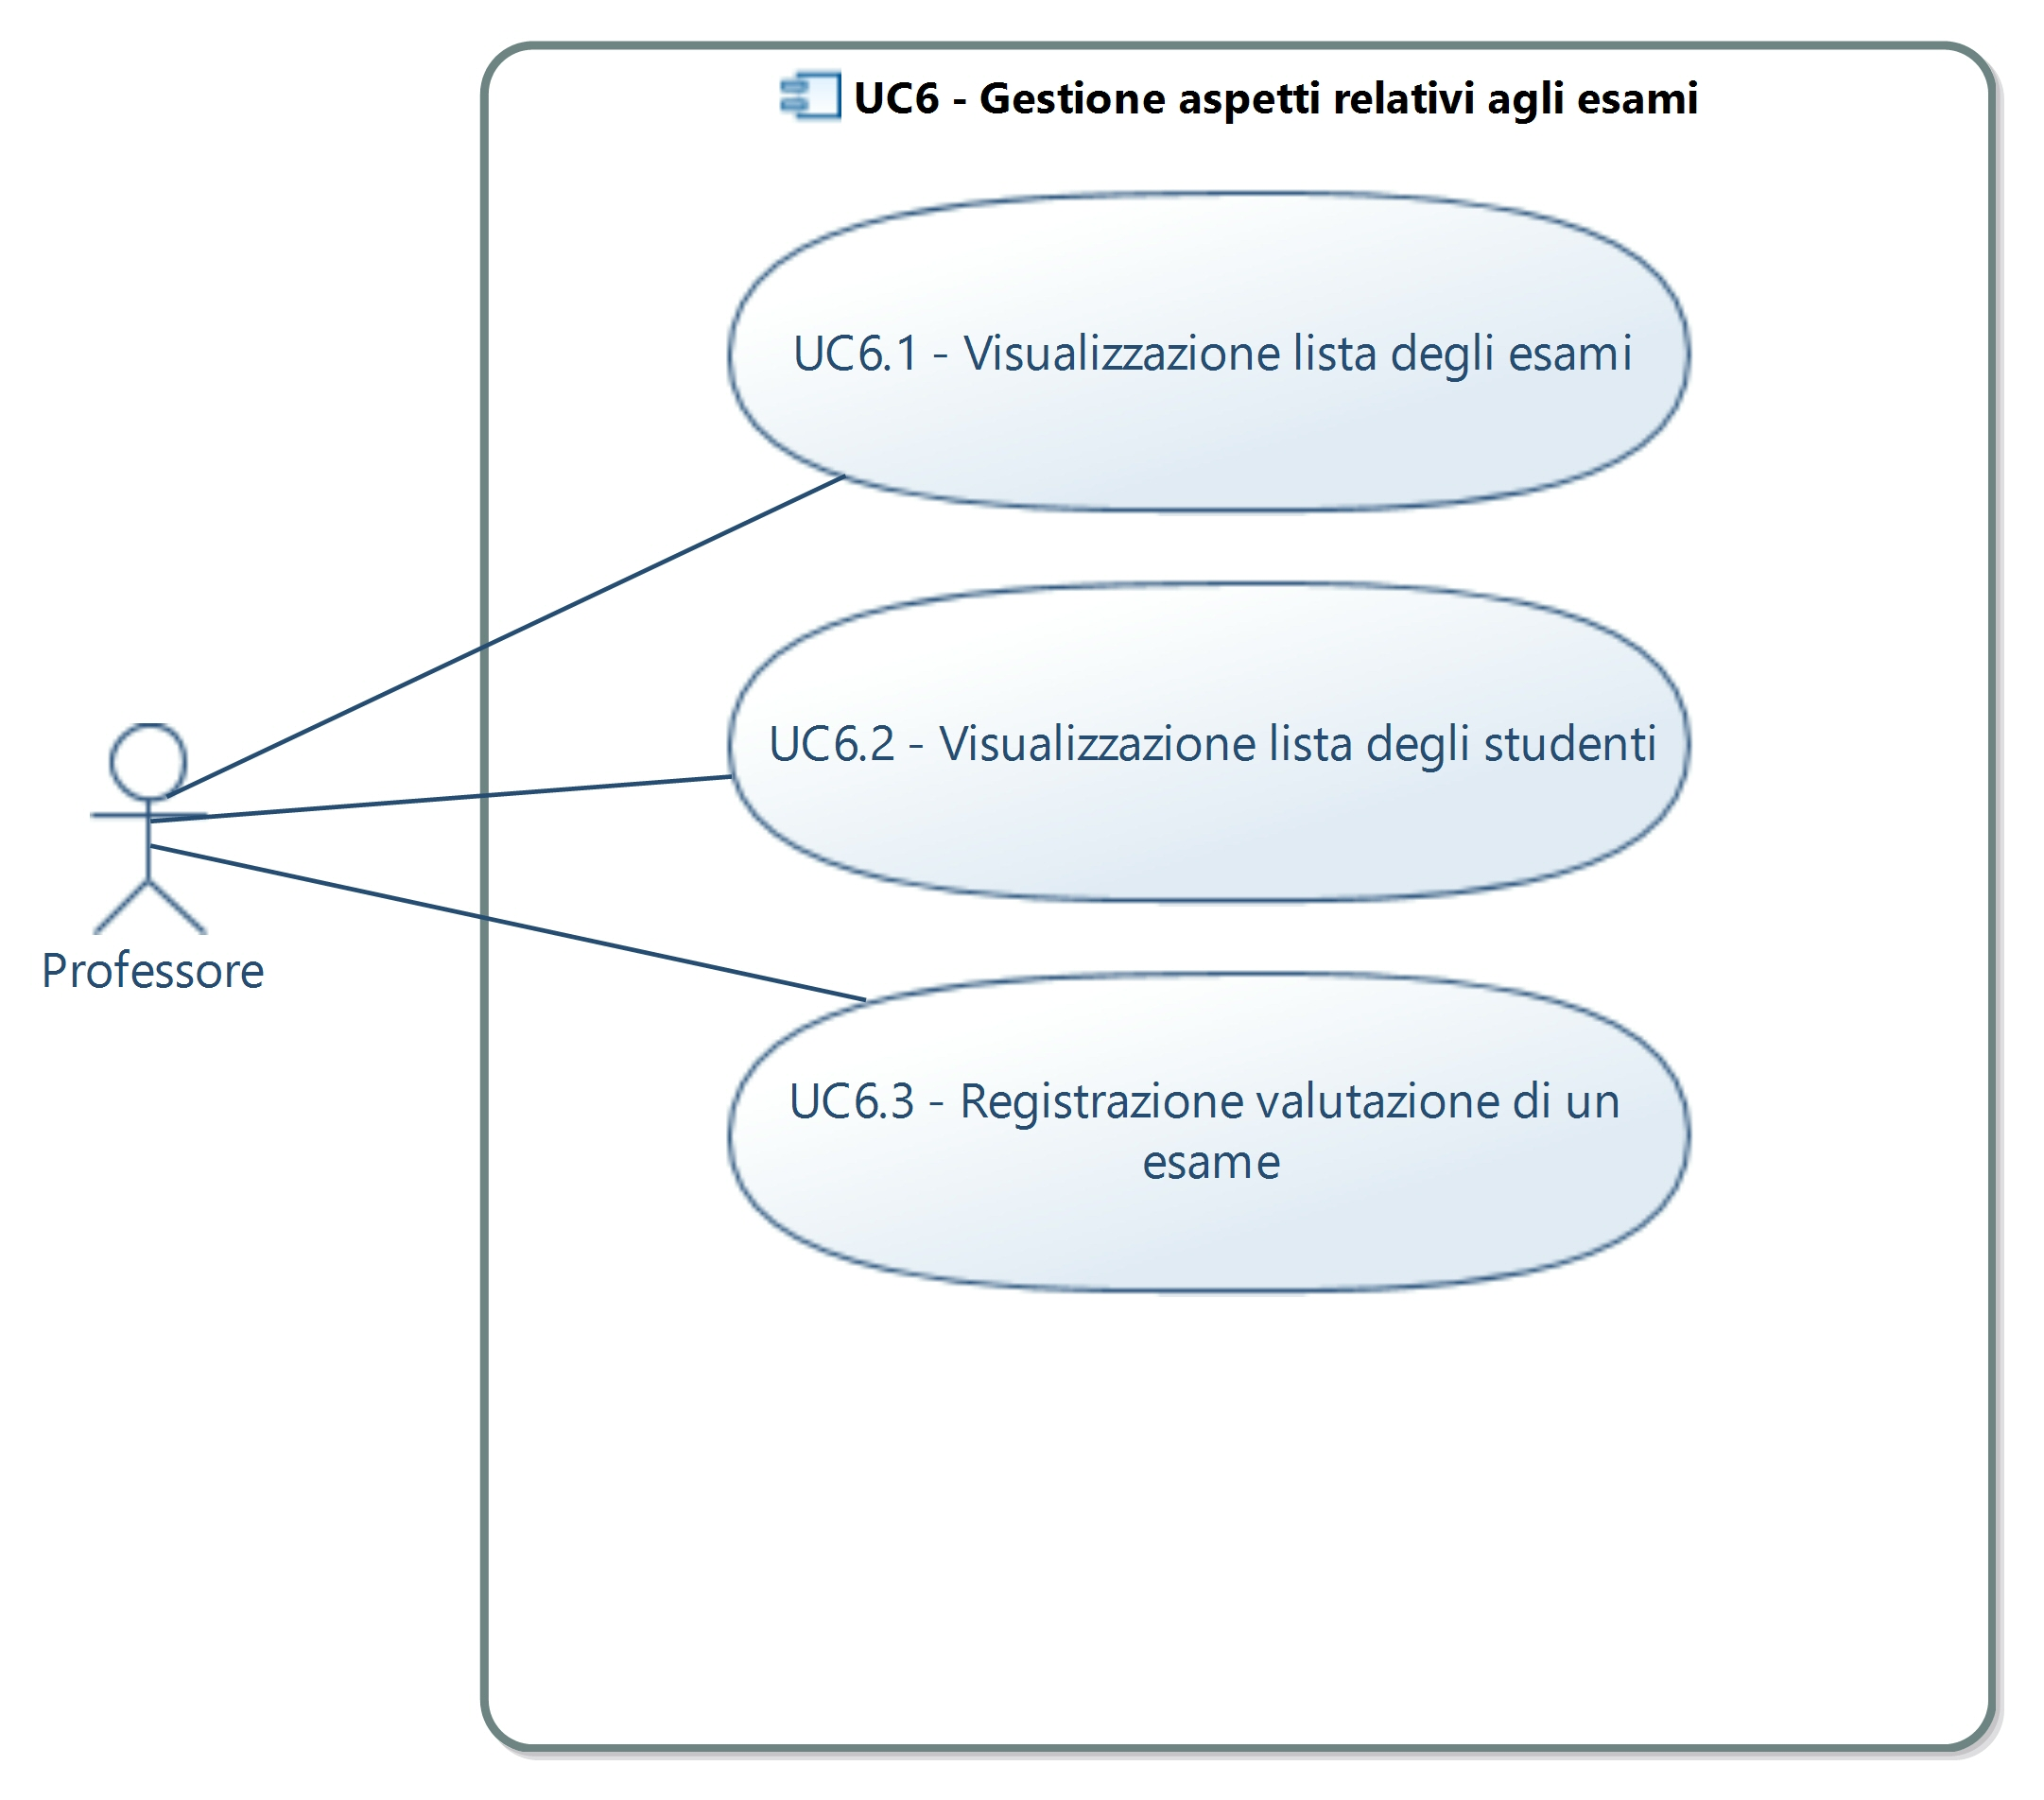
\includegraphics[width=0.8\linewidth]{UC6.jpg}
	\caption{UC6 - Gestione aspetti relativi agli esami}
	\label{fig:UC6 - Gestione aspetti relativi agli esami}
\end{figure}

\subsection{UC6.1 - Visualizzazione lista degli esami}
\begin{itemize}
	\item \textbf{Attori primari:} Professore;\\
	\item \textbf{Scopo e descrizione:} Il professore visualizza una lista di tutti gli esami ai quali è assegnato;\\
	\item \textbf{Scenario principale:} Il professore richiede al sistema la lista degli esami di sua competenza per poterla consultare;\\
	\item \textbf{Precondizione:} L'utente è già riconosciuto dal sistema come professore e richiede la visualizzazione della lista degli esami di sua competenza;\\
	\item \textbf{Postcondizione:} Il professore ottiene la lista degli esami ai quali è assegnato per poterla consultare.\\
\end{itemize}

\subsection{UC6.2 - Visualizzazione lista degli studenti}
\begin{itemize}
	\item \textbf{Attori primari:} Professore;\\
	\item \textbf{Scopo e descrizione:} Il professore visualizza una lista di tutti gli studenti iscritti ad un esame a lui assegnato;\\
	\item \textbf{Scenario principale:} Il professore richiede al sistema la lista degli studenti iscritti ad un esami di sua competenza per poterla consultare;\\
	\item \textbf{Flusso principale degli eventi:}\\
	\begin{enumerate}
		\item Il professore visualizza la lista degli esami di sua competenza [UC6.1];
		\item Il professore, una volta individuato l'esame al quale è interessato, ne richiede la lista degli studenti registrati;
		\item Il professore consulta la lista degli studenti dell'esame richiesto;
	\end{enumerate}
	\item \textbf{Precondizione:} L'utente è già riconosciuto dal sistema come professore e richiede la visualizzazione della lista degli studenti iscritti a un determinato esame di sua competenza;\\
	\item \textbf{Postcondizione:} Il professore ottiene la lista degli studenti iscritti all'esame richiesto per poterla consultare.\\
	%TODO discutere: nessuna estensione, ha la possibilità di richiederlo solo ai suoi corsi, e se manomette il JS comunque non accede a informazioni segrete
\end{itemize}

\subsection{UC6.3 - Registrazione valutazione di un esame}
\begin{itemize}
	\item \textbf{Attori primari:} Professore;\\
	\item \textbf{Scopo e descrizione:} Il professore inserisce nel sistema una valutazione;\\
	\item \textbf{Flusso principale degli eventi:}\\
	\begin{enumerate}
		\item Il professore visualizza la lista degli esami di sua competenza [UC6.1];
		\item Il professore, una volta individuato l'esame al quale è interessato, ne richiede la lista degli studenti registrati [UC6.2];
		\item Il professore consulta la lista degli studenti ed individua la persona alla quale deve inserire la valutazione;
		\item Il professore inserisce la valutazione allo studente;
	\end{enumerate}
	\item \textbf{Precondizione:} Il professore possiede una valutazione da assegnare a uno studente riguardante un determinato esame e desidera registrarlo;\\
	\item \textbf{Postcondizione:} Il voto è stato inserito nella blockchain universitaria.\\
%TODO discutere: nessuna estensione, vede solamente gli studenti dei suoi corsi, non può assegnare voti a studenti a caso di corsi a caso, se cerca di forzarlo modificando il js verrà bloccato dal contratto
\end{itemize}


\subsection{UC7 - Gestione aspetti relativi allo studente}
\begin{itemize}
	\item \textbf{Attori primari:} Studente;\\
	\item \textbf{Scopo e descrizione:} L'utente è già riconosciuto dal sistema come studente e sceglie di utilizzare una funzionalità messa a sua disposizione da parte del sistema;\\
	\item \textbf{Precondizione:} Lo studente già riconosciuto dal sistema desidera effettuare delle operazioni relative alla scelta di esami opzionali o alla visione delle valutazioni;\\
	\item \textbf{Postcondizione:} Lo studente ha visualizzato le operazioni messe a disposizione dal sistema e sceglie quale effettuare.\\
\end{itemize}

\begin{figure}[H]
	\centering
	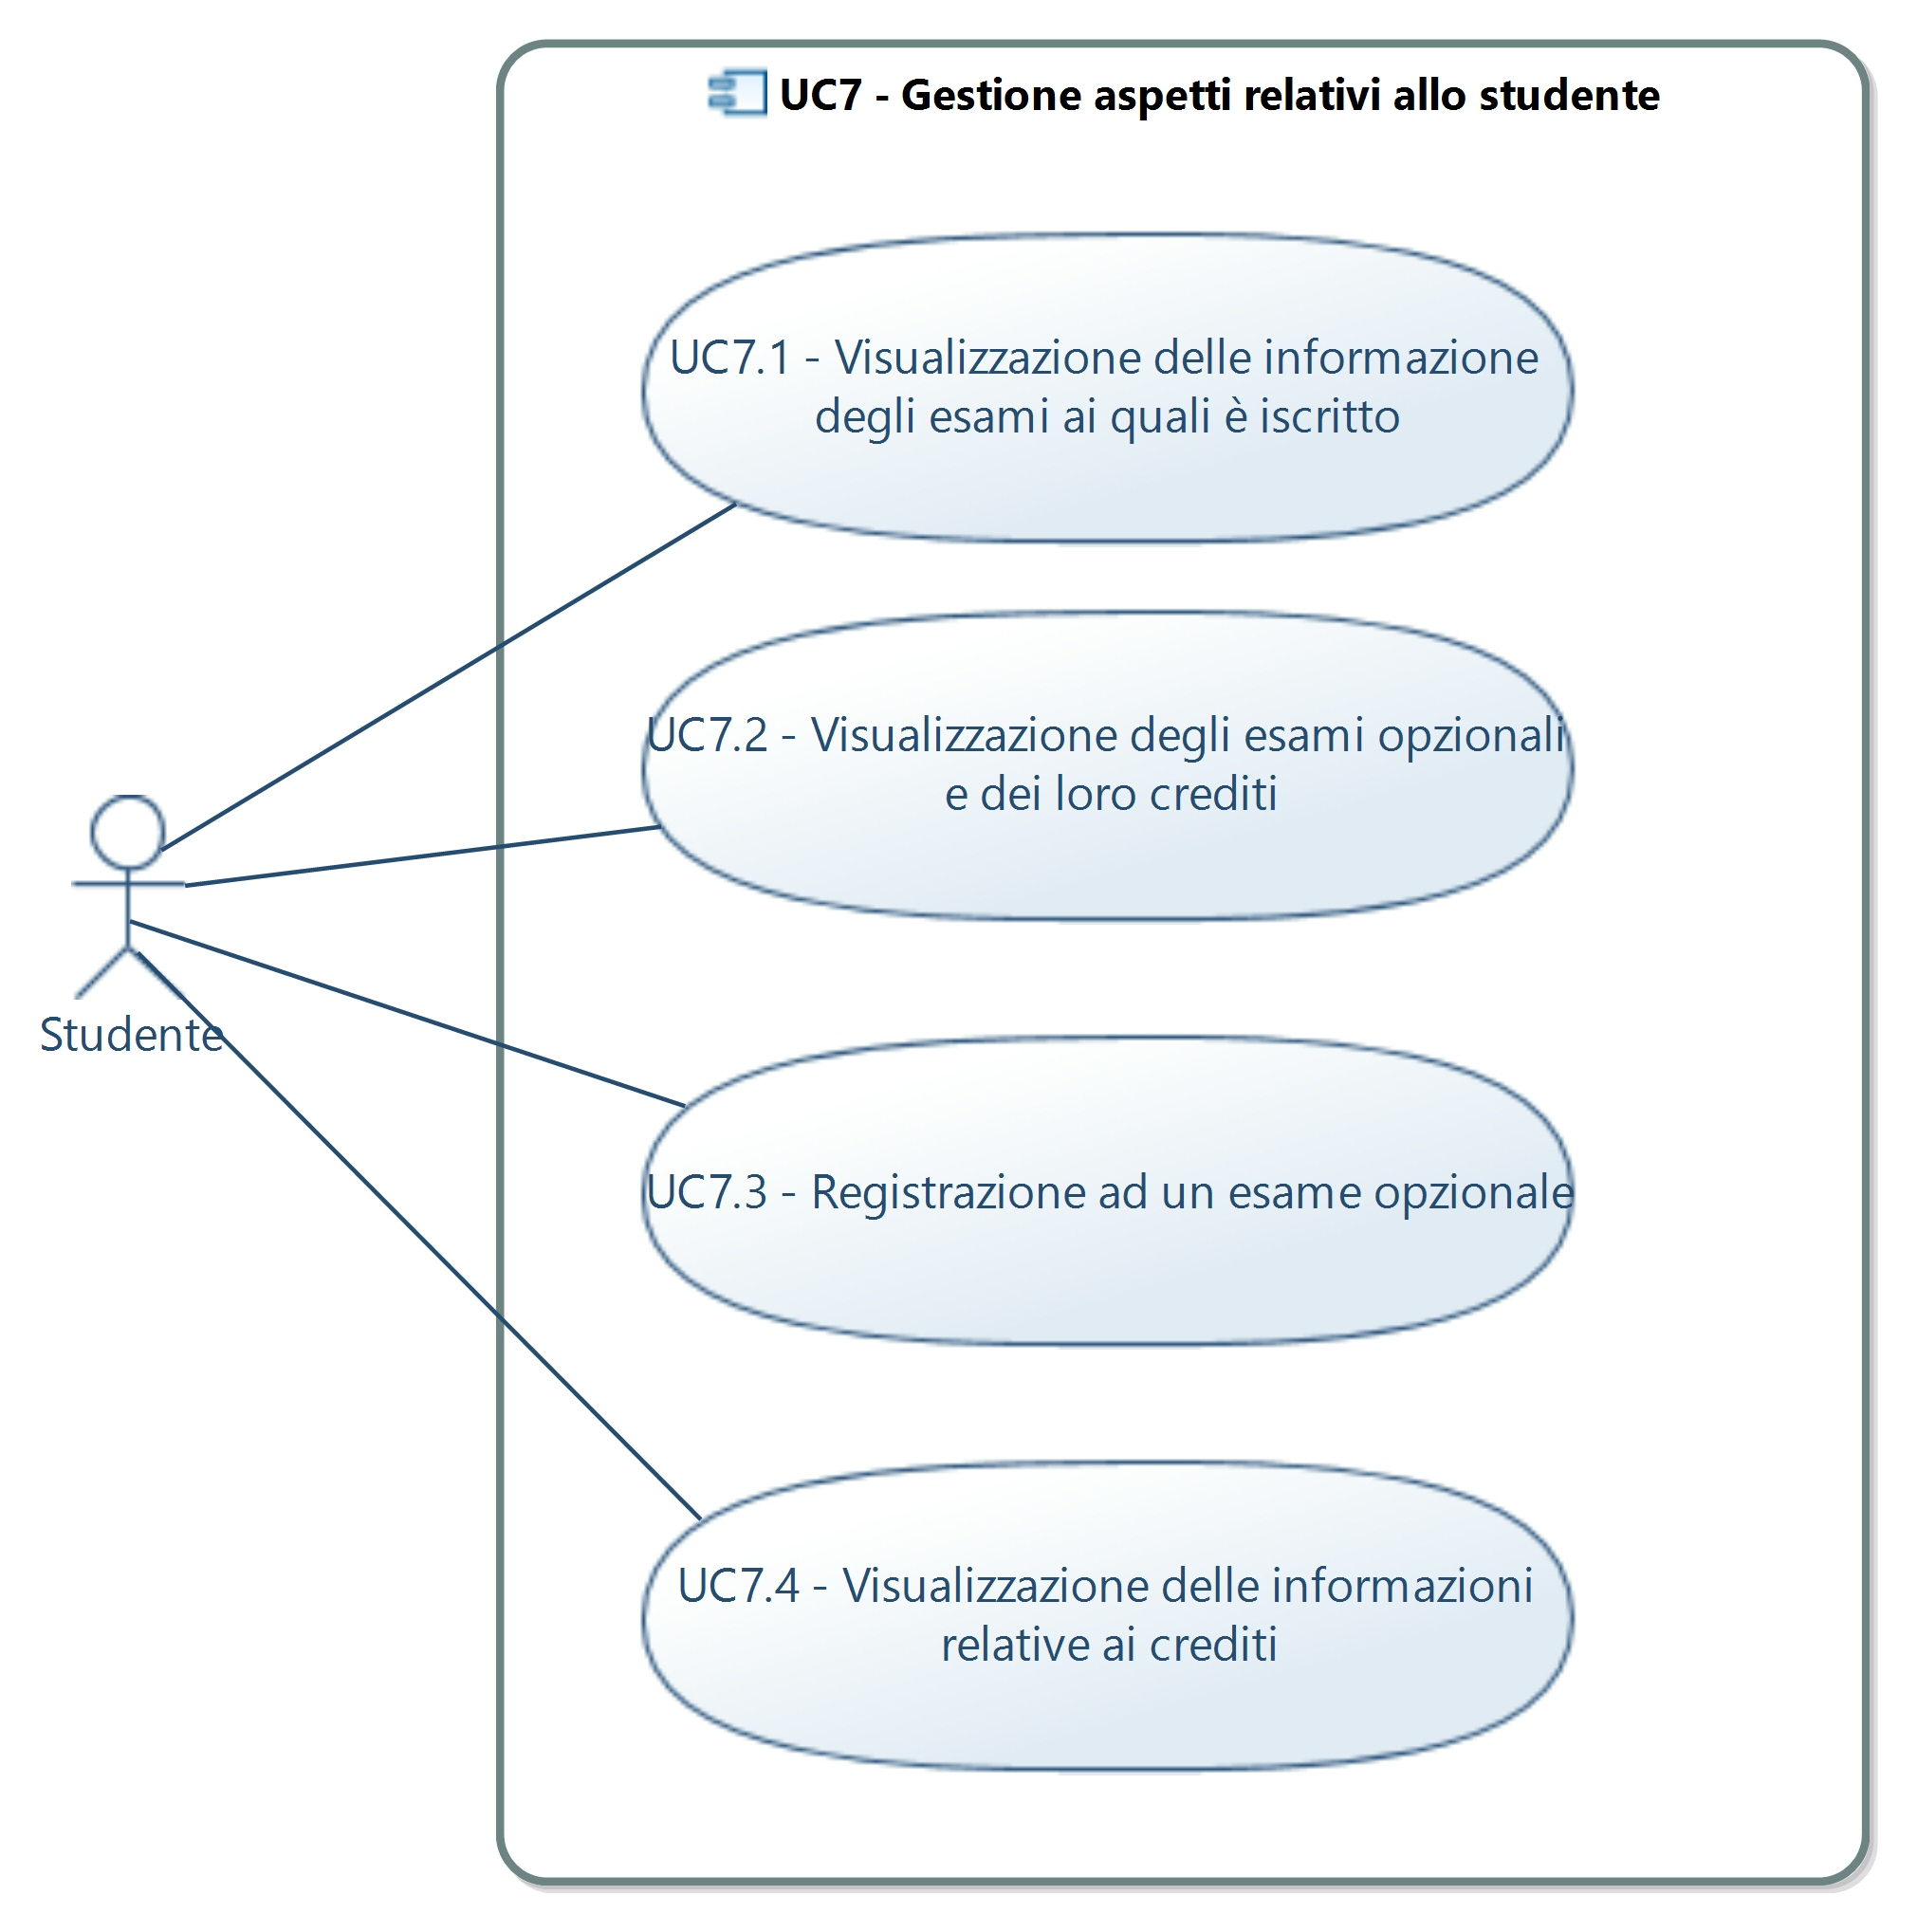
\includegraphics[width=0.8\linewidth]{UC7.jpg}
	\caption{UC7 - Gestione aspetti relativi allo studente}
	\label{fig:UC7 - Gestione aspetti relativi allo studente}
\end{figure}


\subsection{UC7.1 - Visualizzazione delle informazione degli esami ai quali è iscritto}
\begin{itemize}
	\item \textbf{Attori primari:} Studente;\\
	\item \textbf{Scopo e descrizione:} Lo studente visualizza una lista di tutti gli esami ai quali è iscritto;\\
	\item \textbf{Scenario principale:} Lo studente richiede al sistema la lista degli esami ai quali è iscritto per poterla consultare;\\
	\item \textbf{Precondizione:} L'utente è già riconosciuto dal sistema come studente e richiede la visualizzazione della lista degli esami ai quali è iscritto ed le relative informazioni;\\
	\item \textbf{Postcondizione:} Lo studente ottiene la lista per poterla consultare.\\
\end{itemize}

\begin{figure}[H]
	\centering
	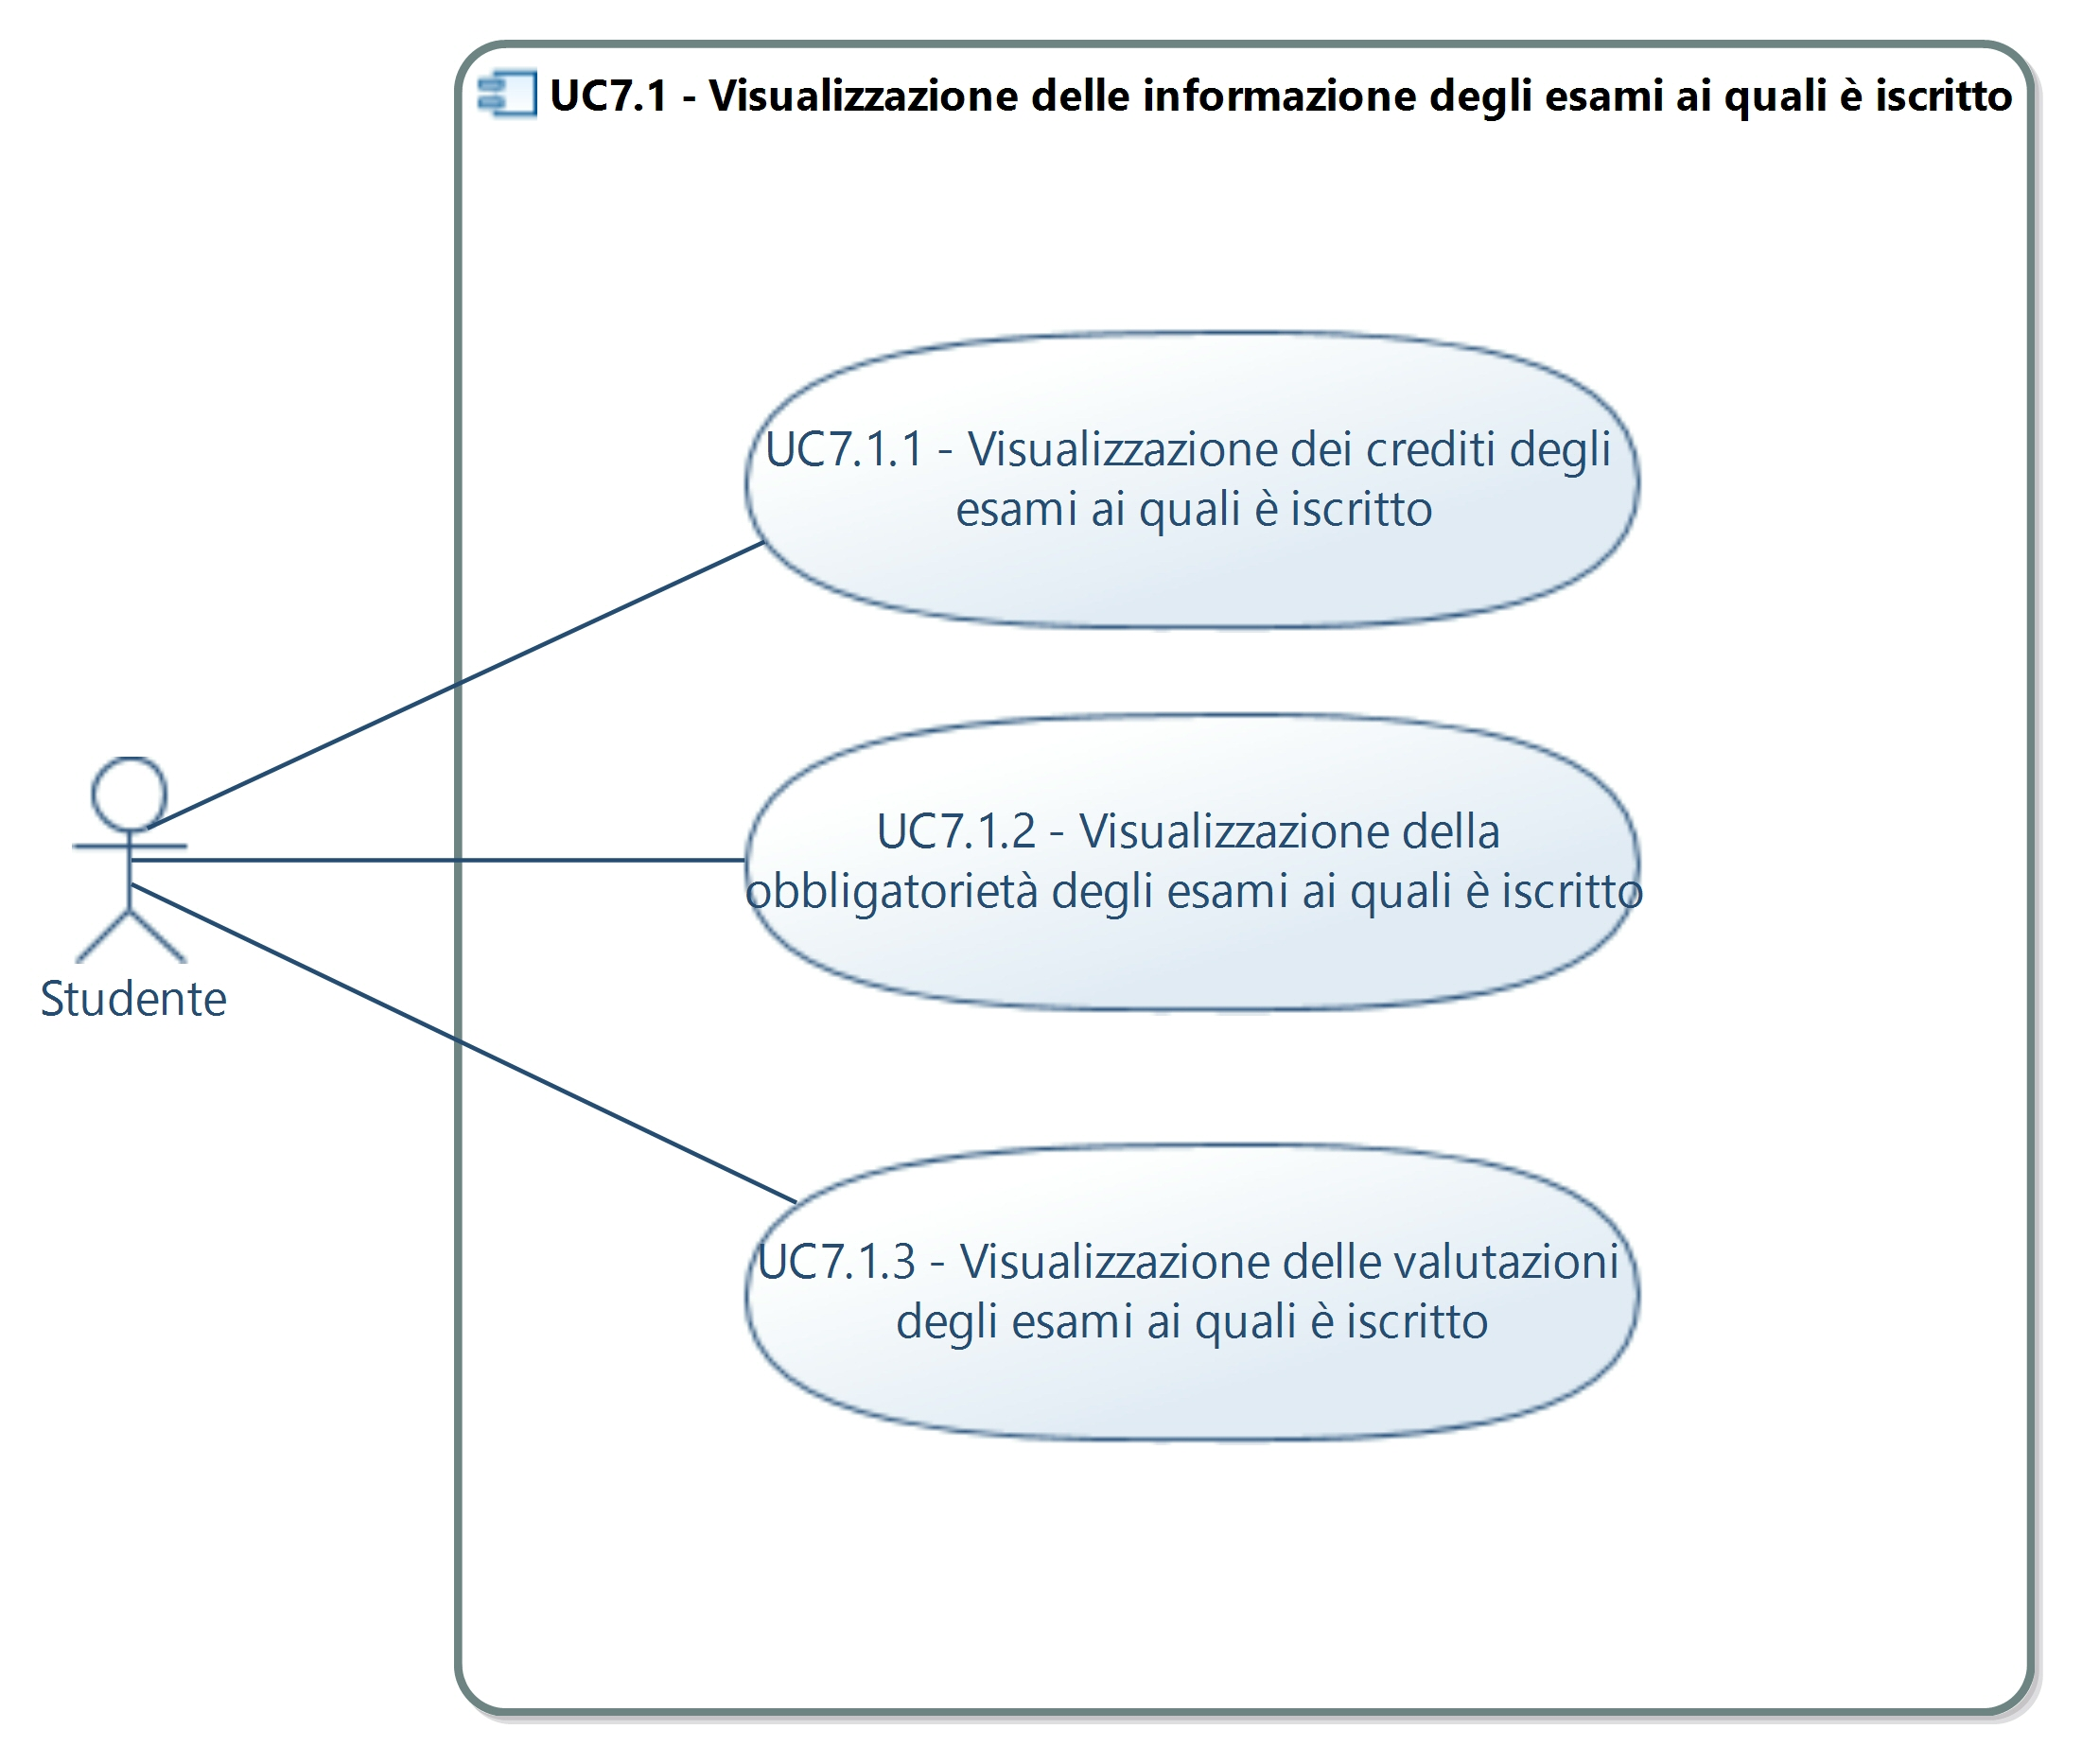
\includegraphics[width=1.0\linewidth]{UC7_1.jpg}
	\caption{UC7.1 - Visualizzazione delle informazione degli esami ai quali è iscritto}
	\label{fig:UC7.1 - Visualizzazione delle informazione degli esami ai quali e' iscritto} %TODO: aggiustare accenti nelle label
\end{figure}

\subsection{UC7.1.1 - Visualizzazione dei crediti degli esami ai quali è iscritto}
\begin{itemize}
\item \textbf{Attori primari:} Studente;\\
\item \textbf{Scopo e descrizione:} Lo studente visualizza il numero di crediti per ogni esame al quale è iscritto;\\
\item \textbf{Scenario principale:} Lo studente richiede al sistema il numero di crediti degli esami ai quali è iscritto per consultarli;\\
\item \textbf{Precondizione:} L'utente è già riconosciuto dal sistema come studente e richiede il numero di crediti per ogni esame ai quale è iscritto;\\
\item \textbf{Postcondizione:} Lo studente ottiene le informazioni richieste.\\
\end{itemize}

\subsection{UC7.1.2 - Visualizzazione della obbligatorietà degli esami ai quali è iscritto}
\begin{itemize}
	\item \textbf{Attori primari:} Studente;\\
	\item \textbf{Scopo e descrizione:} Lo studente visualizza il numero di crediti di per ogni esame al quale è iscritto;\\
	\item \textbf{Scenario principale:} Lo studente richiede al sistema il numero di crediti degli esami ai quali è iscritto per consultarli;\\
	\item \textbf{Precondizione:} L'utente è già riconosciuto dal sistema come studente e richiede il numero di crediti per ogni esame ai quale è iscritto;\\
	\item \textbf{Postcondizione:} Lo studente ottiene le informazioni richieste.\\
\end{itemize}

\subsection{UC7.1.3 - Visualizzazione delle valutazioni degli esami ai quali è iscritto}
\begin{itemize}
	\item \textbf{Attori primari:} Studente;\\
	\item \textbf{Scopo e descrizione:} Lo studente visualizza la valutazione, in formato numerico con l'indicazione di averlo superato se il voto è superiore a 18, per ogni esame al quale è iscritto;\\
	\item \textbf{Scenario principale:} Lo studente richiede al sistema le informazioni riguardanti le valutazioni degli esami ai quali è iscritto per consultarle;\\
	\item \textbf{Precondizione:} L'utente è già riconosciuto dal sistema come studente e richiede le informazioni riguardanti le valutazioni degli esami ai quali è iscritto;\\
	\item \textbf{Postcondizione:} Lo studente ottiene le informazioni richieste.\\
\end{itemize}

\subsection{UC7.2 - Visualizzazione degli esami opzionali e dei loro crediti}
\begin{itemize}
	\item \textbf{Attori primari:} Studente;\\
	\item \textbf{Scopo e descrizione:} Lo studente visualizza una lista di tutti gli esami opzionali ai quali ha possibilità di iscriversi ed i relativi crediti;\\
	\item \textbf{Scenario principale:} Lo studente richiede al sistema la lista di tutti gli esami opzionali ai quali ha possibilità di iscriversi per poterla consultare con i relativi crediti;\\
	\item \textbf{Precondizione:} L'utente è già riconosciuto dal sistema come studente e richiede la visualizzazione della lista di tutti gli esami opzionali ai quali ha possibilità di iscriversi;\\
	\item \textbf{Postcondizione:} Lo studente ottiene la lista per poterla consultare.\\
\end{itemize}

\subsection{UC7.3 - Registrazione ad un esame opzionale}
\begin{itemize}
	\item \textbf{Attori primari:} Studente;\\
	\item \textbf{Scopo e descrizione:} Lo studente si iscrive a un determinato esame opzionale;\\
	\item \textbf{Flusso principale degli eventi:}\\
	\begin{enumerate}
		\item Lo studente visualizza la lista degli esami opzionali [UC7.2];
		\item Lo studente individua l'esame al quale è interessato iscriversi;
		\item Lo studente compie l'operazione di iscrizione;
	\end{enumerate}
	\item \textbf{Precondizione:} Lo studente ha individuato l'esame opzionale al quale desidera iscriversi;\\
	\item \textbf{Postcondizione:} Lo studente inserisce nella blockchain universitaria l'iscrizione all'esame.\\
\end{itemize}

\subsection{UC7.4 - Visualizzazione delle informazioni relative ai crediti}
\begin{itemize}
	\item \textbf{Attori primari:} Studente;\\
	\item \textbf{Scopo e descrizione:} Lo studente visualizza un riepilogo del numero dei crediti che possiede e dell'obiettivo per poter conseguire la laurea;\\
	\item \textbf{Scenario principale:} Lo studente richiede al sistema le informazioni riguardanti i suoi crediti;\\
	\item \textbf{Precondizione:} L'utente è già riconosciuto dal sistema come studente e richiede la visualizzazione delle informazioni relative ai suoi crediti;\\
	\item \textbf{Postcondizione:} Lo studente ottiene le informazioni richieste per poterle consultare.\\
\end{itemize}

\end{document}